\documentclass[10pt]{article}
\usepackage[margin=0.78in]{geometry}
\usepackage{amsmath,amssymb,booktabs,graphicx,microtype,siunitx,xcolor}
\usepackage[hidelinks]{hyperref}
\usepackage{longtable}
\usepackage{enumitem}
\usepackage[section]{placeins}
\graphicspath{{../figures/}}
\sisetup{detect-all,round-mode=places,round-precision=4}

\definecolor{passgreen}{RGB}{0,110,75}
\definecolor{failred}{RGB}{178,34,34}
\newcommand{\PASS}{\textcolor{passgreen}{\textsc{pass}}}
\newcommand{\FAIL}{\textcolor{failred}{\textsc{fail}}}

\title{Recomputed stabilization diagnostics from the validated\\
five-dimensional three-mode stationary density}
\author{Analysis-only audit for Section~4.2}
\date{15 September 2026}

\begin{document}
\maketitle

\begin{abstract}
We recompute the endpoint-exchange asymmetry, energy-conditioned phase
locking, and stationary current balance of the driven three-mode chain from
the normalized five-dimensional NESS density trained on projection-free,
double-precision trajectories.  Every density statistic is restricted to the
predeclared Section~4.1 sampled-support mask and compared with an independent
held-out trajectory estimate and with the legacy neural density.  The new
density reproduces the angular marginal and most locking statistics much more
closely than the legacy density.  Nevertheless, the frozen validation is not a
complete pass: the conservative three-times-floor asymmetry gate fails, three
of thirty phase-locking comparisons have nonoverlapping confidence intervals,
and the masked current balance differs from the trajectory estimate by
$2.31$ bootstrap standard errors.  The global current identity itself passes
on the unconditioned held-out trajectories.  The resulting Section~4.2 claims
must therefore remain support-restricted and diagnostic-specific.
\end{abstract}

\section{Inputs, measures, and frozen gates}

The state is
$x=(I_1,I_2,I_3,\theta_1,\theta_3)$ with density measured against
$dI_1dI_2dI_3d\theta_1d\theta_3$.  We use the fine-step R11 density ensemble
with training seeds $8201$, $8202$, and $8203$; the ensemble is the arithmetic
mean of three separately normalized densities.  The driven case is
$(T_1,T_3)=(2,8)$ and the exact exchange-symmetric control is $(5,5)$.
Uncertainty intervals use $1000$ whole-stream bootstrap replicates with seed
$20260915042$.  The independent V6 test set contains $32$ driven streams
($3{,}200{,}032$ states) and $16$ equilibrium streams ($1{,}600{,}016$
states).

The support mask was fixed from validation trajectories before test
evaluation.  It keeps the central $0.1$--$99.9\%$ action ranges, pools $I_1$
and $I_3$ when setting their bounds so that the mask is exchange invariant,
and retains the full angular torus.  It covers $99.420\%$ of the driven
held-out probability and $99.403\%$ of the equilibrium held-out probability.
The new driven density assigns $99.422\%$ of its mass to the mask; the legacy
density assigns $98.412\%$ and has only $3.37\%$ importance-sampling effective
sample fraction.  No density value is used outside the mask.

For the exchange map
\[
 \sigma(I_1,I_2,I_3,\theta_1,\theta_3)
 =(I_3,I_2,I_1,\theta_3,\theta_1),
\]
we predeclared the pointwise relative asymmetry
\[
 A_\sigma(x)=\frac{|\rho(x)-\rho(\sigma x)|}
 {\rho(x)+\rho(\sigma x)}
\]
and the total-variation asymmetry of a fixed $60\times60$ angular histogram,
$\mathrm{TV}_\sigma=\tfrac12\sum_{ab}|P_{ab}-P_{ba}|$.  The strict
asymmetry gate requires all three driven seeds to exceed the equilibrium
upper bootstrap floor and the driven lower limit to exceed three times that
floor.  Phase locking is evaluated in energy terciles fixed from validation
data, with $72$ periodic angle bins and a fixed half-width $\pi/6$.  A
density/trajectory locking comparison passes only when the two whole-stream
bootstrap intervals overlap.

\section{Endpoint-exchange asymmetry}

\begin{table}[ht]
\centering
\caption{Exchange-asymmetry diagnostics on the support mask.  Brackets give
the percentile range of the resampled histogram estimator.  Because total
variation is nonnegative, this resampling distribution is positively biased
at equilibrium and serves as a conservative measured floor.}
\label{tab:asymmetry}
\small
\begin{tabular}{llrrrrr}
\toprule
case & source & mean $A_\sigma$ & median & p90 & maximum & angular TV \\
\midrule
driven & new density & 0.17961 & 0.11529 & 0.44708 & 0.99894 & 0.11489 [0.11369,0.11959] \\
driven & legacy density & 0.13620 & 0.08257 & 0.35218 & 0.77445 & 0.09920 [0.09690,0.10866] \\
driven & held-out trajectory & -- & -- & -- & -- & 0.11587 [0.11365,0.12120] \\
\addlinespace
equilibrium & new density & $1.30\!\times\!10^{-16}$ & 0 & $4.44\!\times\!10^{-16}$ & $7.11\!\times\!10^{-15}$ & 0.02871 [0.03414,0.04668] \\
equilibrium & legacy density & 0.00633 & 0.00510 & 0.01332 & 0.04368 & 0.03079 [0.03578,0.04916] \\
equilibrium & held-out trajectory & -- & -- & -- & -- & 0.02747 [0.03276,0.04545] \\
\bottomrule
\end{tabular}
\end{table}

The driven new-density angular TV is $4.00$ times the equilibrium point
estimate, and its three seed values lie in the narrow range
$[0.11405,0.11567]$.  It also agrees with the independent held-out value
$0.11587$.  Thus the observed breaking is reproducible and not a legacy-model
effect.  Under the deliberately conservative frozen gate, however, the ratio
of the driven lower limit to the equilibrium upper floor is only $2.435$, not
the required $3$.  The first seed-consistency sub-gate passes, whereas the
three-times-floor sub-gate \FAIL.  This result must be reported as a failed
formal gate, not converted into a pass by changing the threshold.

\begin{figure}[ht]
\centering
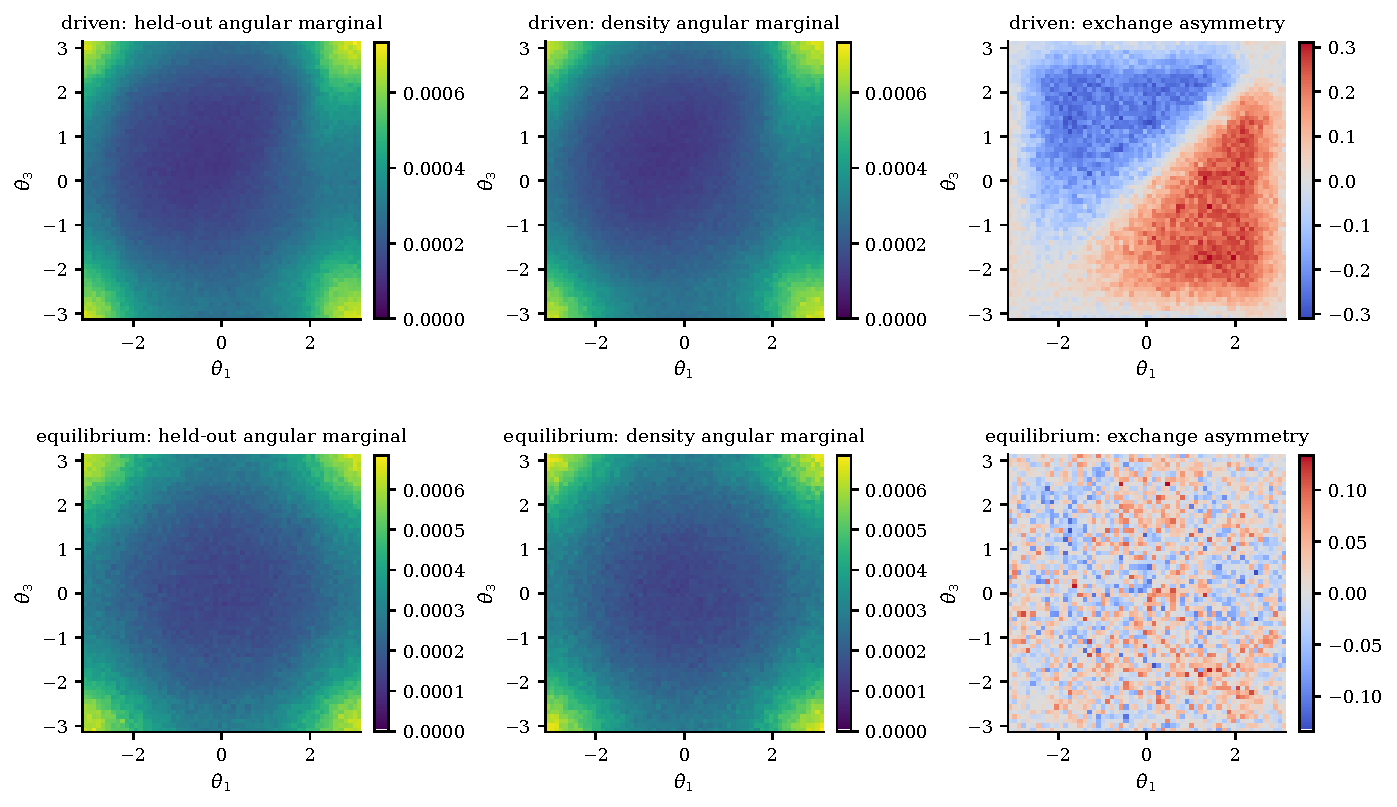
\includegraphics[width=\textwidth]{exchange_asymmetry_rebuilt.pdf}
\caption{Angular marginals and endpoint-exchange asymmetry.  The driven
validated density closely tracks the held-out trajectory marginal and exhibits
a coherent antisymmetric structure.  The equilibrium panel shows the finite
histogram floor rather than physical symmetry breaking.}
\label{fig:exchange}
\end{figure}

\section{Energy-conditioned phase locking}

The high-energy branch used without tuning is
\[
 \theta_0=\pi-\arcsin\!\left[
 \frac{\sqrt{4\gamma^2+3}-\gamma}{2(1+\gamma^2)}\right]
 =2.19120\ \mathrm{rad}=125.547^\circ,
\]
with $\gamma=0.1$.  Table~\ref{tab:locking} gives representative fixed-window
probabilities.  The complete $360$-row table, including circular means,
resultants, histogram modes, all three model seeds, both physical cases, and
the legacy density, is supplied as \texttt{analysis/phase\_locking.csv}.

\begin{table}[ht]
\centering
\caption{Driven conditional locking probabilities.  Columns are held-out
trajectory / validated density / legacy density.  The first row in each
sector is $P(|\theta_1-\theta_0|<\pi/6)$, the second is
$P(|\theta_3+2\pi/3|<\pi/6)$, and the third requires both angles to lie near
$\theta_0$.}
\label{tab:locking}
\small
\begin{tabular}{llrrr}
\toprule
energy & statistic & held-out & new density & legacy density \\
\midrule
low & $\theta_1$ near $\theta_0$ & 0.20413 & 0.20432 & 0.20060 \\
low & $\theta_3$ near $-2\pi/3$ & 0.19329 & 0.19378 & 0.19146 \\
low & both near $\theta_0$ & 0.03906 & 0.03819 & 0.03750 \\
\addlinespace
middle & $\theta_1$ near $\theta_0$ & 0.21739 & 0.21840 & 0.21150 \\
middle & $\theta_3$ near $-2\pi/3$ & 0.20279 & 0.20505 & 0.20104 \\
middle & both near $\theta_0$ & 0.03984 & 0.03928 & 0.03769 \\
\addlinespace
high & $\theta_1$ near $\theta_0$ & 0.25047 & 0.24469 & 0.22301 \\
high & $\theta_3$ near $-2\pi/3$ & 0.21893 & 0.21817 & 0.20742 \\
high & both near $\theta_0$ & 0.04206 & 0.04182 & 0.03842 \\
\bottomrule
\end{tabular}
\end{table}

The rebuilt density agrees with the direct estimate in $27$ of $30$
predeclared driven comparisons.  The three failures are retained in
Table~\ref{tab:phasefail}.  Their absolute discrepancies are small but
statistically resolved by the large held-out sample.  In particular, the
high-energy $\theta_1$ locking probability moves from $0.22301$ under the
legacy density to $0.24469$ under the new density, substantially closer to the
direct $0.25047$, but its intervals still do not overlap.

\begin{table}[ht]
\centering
\caption{All failed new-density versus held-out phase comparisons.}
\label{tab:phasefail}
\small
\begin{tabular}{llllrrr}
\toprule
sector & angle & statistic & density [95\%] & trajectory [95\%] & difference & $z_{\rm approx}$ \\
\midrule
low & $\theta_3$ & circular mean & $-3.0299$ [$-3.0549$,$-3.0077$] & $-3.0650$ [$-3.0828$,$-3.0444$] & 0.03514 & 2.26 \\
middle & $\theta_1$ & circular mean & 2.8894 [2.8698,2.9084] & 2.9194 [2.8997,2.9360] & $-0.02999$ & $-2.21$ \\
high & $\theta_1$ & locking probability & 0.24469 [0.24258,0.24706] & 0.25047 [0.24800,0.25332] & $-0.00578$ & $-3.26$ \\
\bottomrule
\end{tabular}
\end{table}

\begin{figure}[ht]
\centering
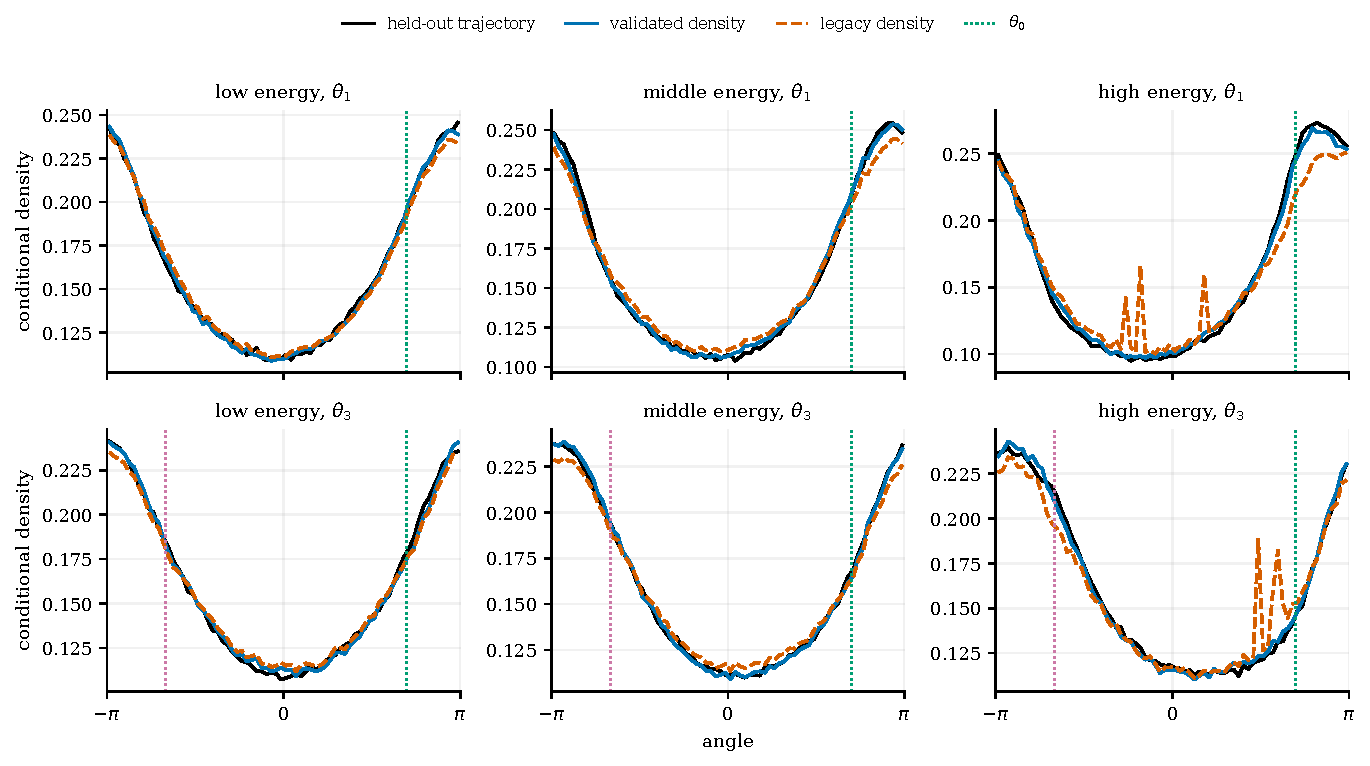
\includegraphics[width=\textwidth]{phase_locking_rebuilt.pdf}
\caption{Driven angular distributions conditioned on validation-fixed energy
terciles.  The validated density follows the held-out curves closely; the
legacy density exhibits visible high-energy sampling noise and larger
departures.  Vertical lines mark the fixed high- and low-energy references.}
\label{fig:locking}
\end{figure}

\section{Current balance and scope audit}

For the middle action, the state observables are
\[
 J_{12}=I_1I_2\sin\theta_1,\qquad
 J_{23}=I_2I_3\sin\theta_3.
\]
Stationarity implies the \emph{unconditioned} identity
$\langle J_{12}+J_{23}\rangle=0$.  The original frozen protocol mistakenly
required this identity after conditioning on the support mask.  That
conditioned expectation need not vanish because the mask introduces a
selection boundary.  We preserve the original result and add a post-hoc scope
audit rather than silently changing it.

\begin{table}[ht]
\centering
\caption{Driven current estimates on the common support mask.  These values
test density reconstruction, not the unconditioned zero identity.}
\label{tab:maskedcurrent}
\small
\begin{tabular}{lrrr}
\toprule
source & $\langle J_{12}\rangle$ & $\langle J_{23}\rangle$ & sum \\
\midrule
held-out trajectory & 0.23057 [0.22607,0.23501] & $-0.22865$ [$-0.23297$,$-0.22408$] & 0.001926 [0.001321,0.002552] \\
new density & 0.23136 [0.22549,0.23709] & $-0.23520$ [$-0.24241$,$-0.22808$] & $-0.003847$ [$-0.008807$,0.000529] \\
legacy density & 0.16834 [0.11436,0.20334] & $-0.04459$ [$-0.19573$,0.14779] & 0.12375 [$-0.00319$,0.30034] \\
\bottomrule
\end{tabular}
\end{table}

The masked new-density sum differs from the identically masked held-out sum by
$-0.005773$, or $-2.306$ bootstrap standard errors.  The applicable
density/trajectory gate therefore \FAIL.  The equilibrium masked comparison
passes at $0.586$ standard errors.

On the complete held-out driven trajectories, by contrast,
\[
 \langle J_{12}\rangle=0.2327497,
 \quad \langle J_{23}\rangle=-0.2327327,
 \quad \langle J_{12}+J_{23}\rangle
 =1.7046\times10^{-5},
\]
with a whole-stream $95\%$ interval
$[-2.7013\times10^{-4},3.1681\times10^{-4}]$ and $z=0.116$.
The equilibrium complete-trajectory sum is $9.1214\times10^{-5}$ with interval
$[-3.1739\times10^{-4},5.3720\times10^{-4}]$ and $z=0.411$.  Thus the physical
stationary current identity passes in both cases.  We do not extrapolate the
density outside its validated support to manufacture a global density result.

\begin{figure}[ht]
\centering
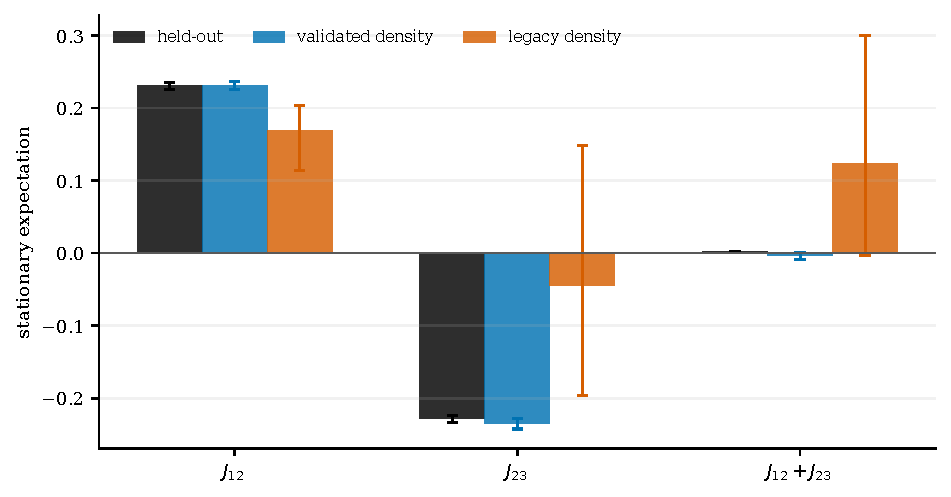
\includegraphics[width=0.82\textwidth]{current_balance_rebuilt.pdf}
\caption{Current expectations on the Section~4.1 support mask.  The new
density reproduces the two directed currents far better than the legacy
density, but its current sum remains $2.31$ standard errors from the masked
held-out value.}
\label{fig:current}
\end{figure}

\section{Gate ledger and claim boundary}

\begin{table}[ht]
\centering
\caption{Frozen and scope-audited gates.}
\label{tab:gates}
\small
\begin{tabular}{p{0.58\textwidth}rrl}
\toprule
gate & observed & reference & result \\
\midrule
minimum driven seed TV exceeds equilibrium upper floor & 0.11405 & 0.04668 & \PASS \\
driven lower TV exceeds three times equilibrium upper floor & 0.11369 & 0.14005 & \FAIL \\
phase density/trajectory interval overlaps & 27/30 & 30/30 & \FAIL \\
masked current difference $|z|\le1.96$ & 2.306 & 1.96 & \FAIL \\
global driven held-out current sum contains zero & $1.70\times10^{-5}$ & 0 & \PASS \\
\bottomrule
\end{tabular}
\end{table}

The legacy qualitative picture survives: the temperature gradient produces a
reproducible endpoint-exchange asymmetry, phase locking strengthens with
energy, and stationary transport balances the two bonds globally.  The new
density gives quantitatively closer estimates than the earlier unnormalized
network, especially in the high-energy phase sector and for the directed
currents.  However, the rebuilt Section~4.2 is not fully density-validated
under its frozen gates.  Publication wording should distinguish direct
trajectory results from density-derived reconstruction and explicitly report
the three phase failures and the masked-current discrepancy.  Claims apply
only to the $\approx99.4\%$ sampled-support region.

\section{Reproducibility and provenance}

No simulation or retraining was performed.  The commands were
\begin{verbatim}
./run_analysis.sh
./run_current_scope_audit.sh
./run_report_summary.sh
\end{verbatim}
from
\texttt{experiments/short\_chain\_stabilization\_density\_rebuild\_2026-09-15}.
The source snapshot and analysis hashes are
\begingroup\scriptsize
\begin{verbatim}
source snapshot: 55c6670640bd7c686f1b3704dfa003c0b793ef4d
core analysis:   31c4288612631fdd092dd6688f6267d9cf4fd9a5617a8ec57ac5f0269cdda192
scope audit:     d7e48ff24dcfec856e2743199bf24bd05c9a20b7eb4fc26d99b5a8405028c988
\end{verbatim}
\endgroup

\end{document}
